%% LyX 2.3.6 created this file.  For more info, see http://www.lyx.org/.
%% Do not edit unless you really know what you are doing.
\documentclass[english,xcolor=svgnames, handout]{beamer}
\usepackage{mathpazo}
\usepackage[T1]{fontenc}
\usepackage[latin9]{inputenc}
\setcounter{secnumdepth}{3}
\setcounter{tocdepth}{3}
\usepackage{babel}
\usepackage{calc}
\usepackage{amstext}
\usepackage{graphicx}
\ifx\hypersetup\undefined
  \AtBeginDocument{%
    \hypersetup{unicode=true}
  }
\else
  \hypersetup{unicode=true}
\fi

\makeatletter
%%%%%%%%%%%%%%%%%%%%%%%%%%%%%% Textclass specific LaTeX commands.
% this default might be overridden by plain title style
\newcommand\makebeamertitle{\frame{\maketitle}}%
% (ERT) argument for the TOC
\AtBeginDocument{%
  \let\origtableofcontents=\tableofcontents
  \def\tableofcontents{\@ifnextchar[{\origtableofcontents}{\gobbletableofcontents}}
  \def\gobbletableofcontents#1{\origtableofcontents}
}

%%%%%%%%%%%%%%%%%%%%%%%%%%%%%% User specified LaTeX commands.

% you can play with different themes and color themes to find your favorite combination.
\mode<presentation> {
  \usetheme{Luebeck}
  \usecolortheme{beaver}
  \beamertemplatenavigationsymbolsempty
}


\usepackage{graphicx} % for including images
\usepackage{pgf} % for logo
\usepackage{colortbl}

\date{} % Date, can be changed to a custom date

\titlegraphic{
\vspace{-0.6cm}

\includegraphics[width=1.5cm]{/misc/LogoBlueJustRing.jpg}\break

\tiny
\vspace{1cm}

\includegraphics[width=0.33cm]{/misc/web.png} \href{https://mattiasvillani.com}{mattiasvillani.com}\hspace*{1cm}~

\includegraphics[width=0.3cm]{/misc/twitter.jpg} \href{https://twitter.com/matvil}{@matvil}\hspace*{1cm}~

\includegraphics[width=0.3cm]{/misc/github.png} \href{https://github.com/mattiasvillani}{mattiasvillani}~
}


\definecolor{blue}{RGB}{38, 122, 181}
\definecolor{orange}{RGB}{255, 128, 0}
\definecolor{lorange}{RGB}{255, 178, 102}
\definecolor{llorange}{RGB}{255, 229,204 }
\definecolor{verylightgray}{RGB}{246, 246, 246}


\setbeamertemplate{itemize item}{\color{orange}$\blacksquare$}
\setbeamertemplate{itemize subitem}{\color{orange}$\blacktriangleright$}

\usepackage{tcolorbox}

\newcommand\blfootnote[1]{%
  \begingroup
  \renewcommand\thefootnote{}\footnote{#1}%
  \addtocounter{footnote}{-1}%
  \endgroup
}

\makeatother

\begin{document}
\title[\textcolor{gray}{ST1101 \hspace{4.45cm}\insertframenumber/\inserttotalframenumber}]{\textcolor{orange}{Statistik och Dataanalys I}}
\subtitle{\textcolor{orange}{F�rel�sning 13 - Betingade sannolikheter och Bayes
sats}}
\author[\textbf{\textcolor{gray}{Statistik och Dataanalys I}}]{\textbf{Mattias Villani} \\
\vspace{0.2cm}
\includegraphics[scale=0.02]{\string"misc/Beard Man Emoji\string".eps}\vspace{-0.3cm}
}
\institute[Stockholms universitet]{Statistiska institutionen\\
Stockholms universitet}

\makebeamertitle

\begin{frame}{\textbf{\textcolor{orange}{�versikt}}}
\begin{itemize}
\item \textbf{\textcolor{blue}{Betingade sannolikheter}}
\end{itemize}
\bigskip{}

\begin{itemize}
\item \textbf{\textcolor{blue}{Bayes sats}}
\end{itemize}
\end{frame}

\begin{frame}{\textbf{\textcolor{orange}{Bayes sats - enkel version}}}
\begin{center}
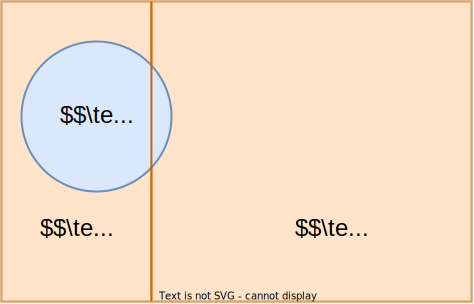
\includegraphics[scale=0.27]{figs/bayes_twoevents}
\par\end{center}
\begin{itemize}
\item Exempel: B = \{har Covid\}. A = \{positivt hemtest\}.
\end{itemize}
\end{frame}

\begin{frame}{\textbf{\textcolor{orange}{Bayes sats - enkel version}}}
\begin{center}
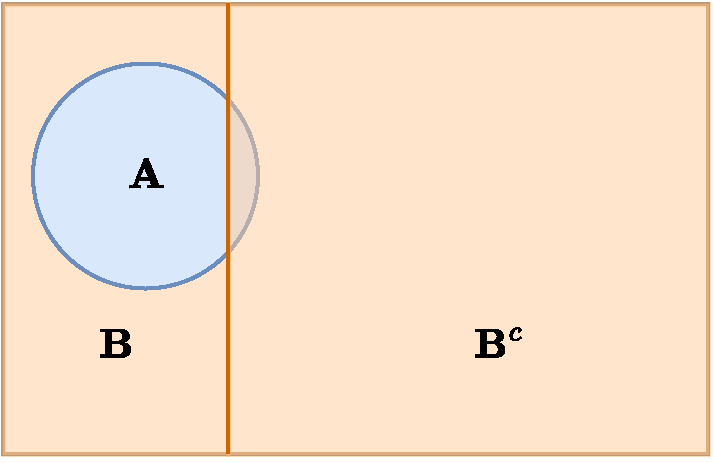
\includegraphics[scale=0.27]{figs/bayes_twoevents_cond}
\[
P(B|A)=\frac{P(A\cap B)}{P(A)}
\]
\par\end{center}

\end{frame}

\begin{frame}{\textbf{\textcolor{orange}{Bayes sats - allm�n version}}}
\begin{center}
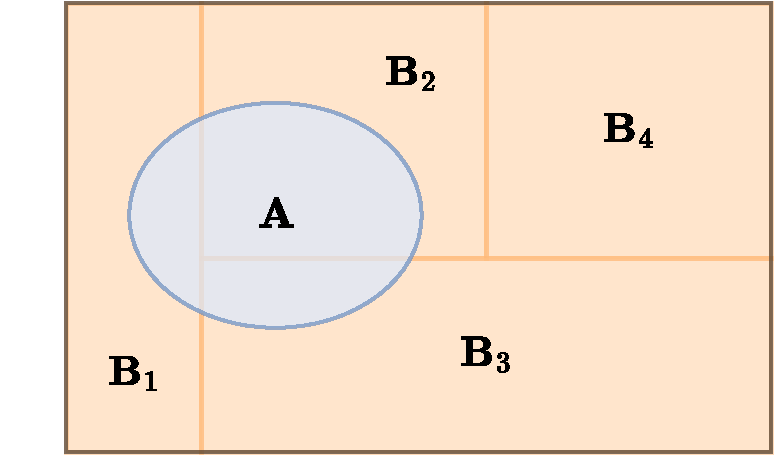
\includegraphics[scale=0.27]{figs/bayesgeneral}
\par\end{center}

\[
P(A)=\sum_{j=1}^{K}P(A|B_{j})p(B_{j})
\]

\end{frame}

\begin{frame}{\textbf{\textcolor{orange}{Bayes sats - allm�n version}}}
\begin{center}
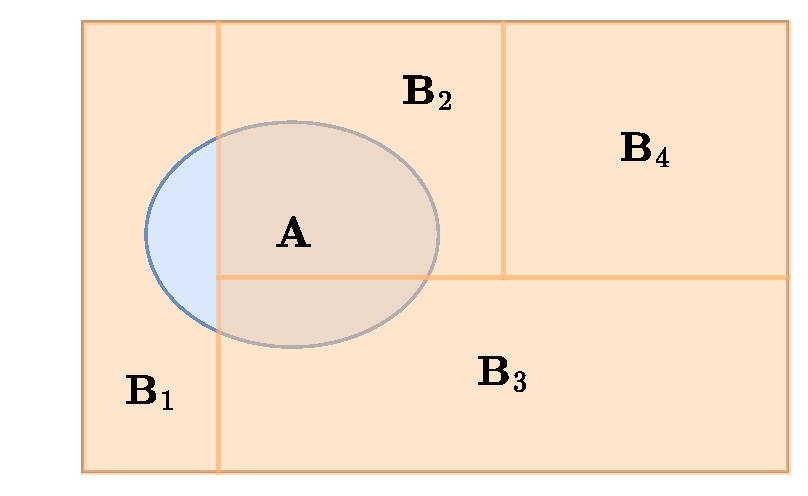
\includegraphics[scale=0.27]{figs/bayesgeneralwithintersect}
\par\end{center}

\[
P(A)=\sum_{j=1}^{K}P(A|B_{j})p(B_{j})
\]

\[
P(B_{k}|A)=\frac{P(A|B_{k})P(B_{k})}{\sum_{j=1}^{K}P(A|B_{j})p(B_{j})}
\]

\end{frame}

\begin{frame}{\textbf{\textcolor{orange}{Funkar hemtest f�r covid?}}}
\begin{center}
\noindent{\fboxrule 1pt\fboxsep 1pt\fcolorbox{orange}{white}{\begin{minipage}[t]{1\columnwidth - 2\fboxsep - 2\fboxrule}%
\begin{center}
\href{https://statisticssu.github.io/SDA1/observable/bayestheorem.html}{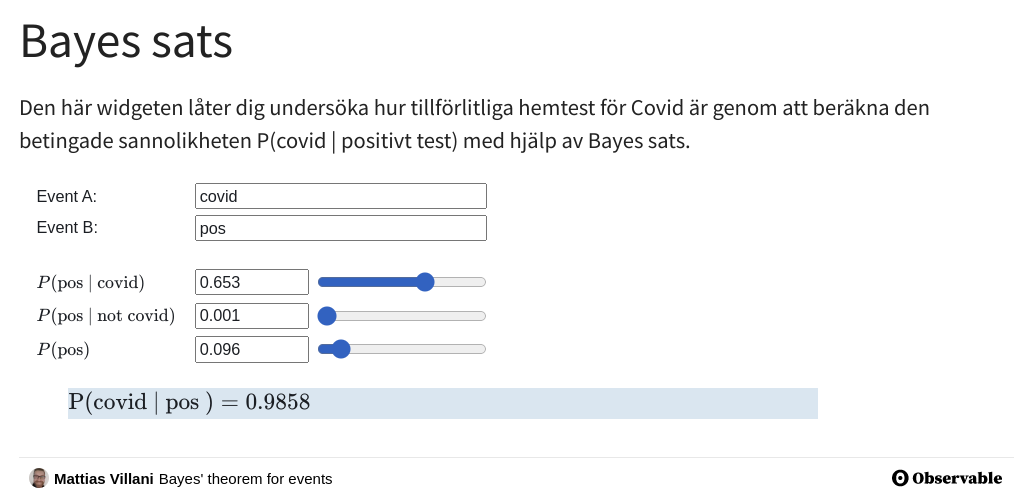
\includegraphics[width=0.9\textwidth]{figs/BayesSatsWidget.png}}
\par\end{center}%
\end{minipage}}}
\par\end{center}

\end{frame}

\begin{frame}{\textbf{\textcolor{orange}{K�nna igen handskrivna siffror}}}
\begin{itemize}
\item $A=$\{svart pixel i mitten\}
\item $B_{0}=$\{siffran �r en nolla\} och $B_{1}=$ \{siffran �r en etta\}
\item M�l: $P(\text{siffran �r en nolla}|\text{svart pixel i mitten})$
\[
P(B_{0}\vert A)=\frac{P(A\vert B_{0})p(B_{0})}{P(A)}
\]
\item Beh�ver veta
\[
p(B_{0})=\frac{1}{10}
\]
\[
P(A)=\frac{\text{antal bilder med svart pixel i mitten}}{\text{totalt antal bilder}}
\]
\[
P(A\vert B_{0})=\frac{\text{andelen bilder med svart pixel i mitten}}{\text{antal bilder med nollor p�}}
\]
\end{itemize}
\begin{center}
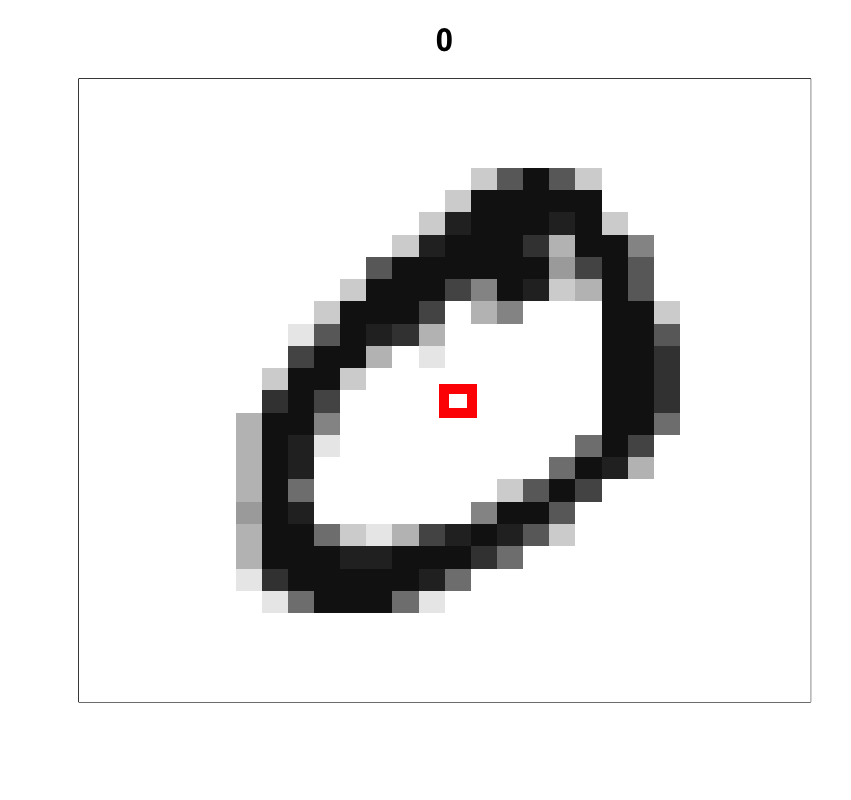
\includegraphics[scale=0.09]{figs/mnistZeroWithRedVoxel}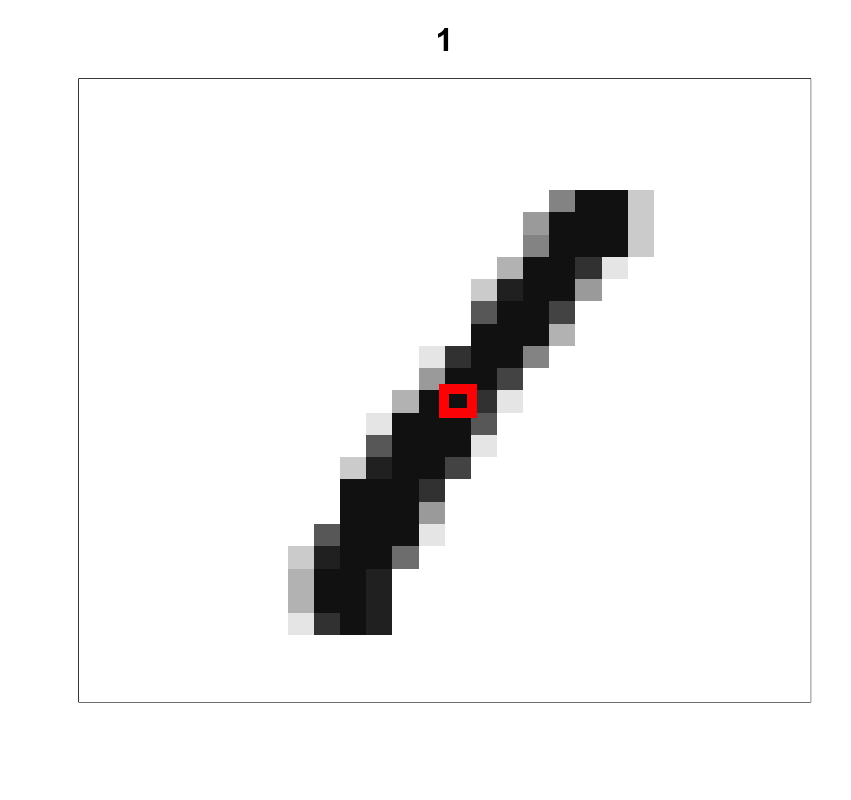
\includegraphics[scale=0.09]{figs/mnistOneWithRedVoxel}
\par\end{center}
\end{frame}

\end{document}
